\documentclass[tikz,border=0pt]{standalone}
\usepackage[T1]{fontenc}
\usepackage{lmodern}
\usepackage{amsmath,amssymb}
\usepackage{xcolor}
\usetikzlibrary{arrows.meta,calc,positioning}

\ifdefined\pdfoutput
  \ifnum\pdfoutput>0
    \ifdefined\pdfinfoomitdate
      \pdfinfoomitdate=1
    \fi
    \ifdefined\pdftrailerid
      \pdftrailerid{}
    \fi
    \ifdefined\pdfsuppressptexinfo
      \pdfsuppressptexinfo=15
    \fi
  \fi
\fi

\definecolor{ink}{HTML}{17212B}
\definecolor{muted}{HTML}{52606D}
\definecolor{line}{HTML}{C9D2DA}
\definecolor{panel}{HTML}{F7F9FB}
\definecolor{radial}{HTML}{176B9A}
\definecolor{azimuthal}{HTML}{B85C00}
\definecolor{positive}{HTML}{1F6E43}
\definecolor{positivefill}{HTML}{E8F4EC}
\definecolor{note}{HTML}{EEF3F6}

\tikzset{
  component arrow/.style={line width=1.25pt,-{Latex[length=3.6mm,width=2.5mm]}},
  case panel/.style={draw=line,line width=.65pt,rounded corners=2.5mm,fill=panel},
  result box/.style={draw=positive!55,line width=.65pt,rounded corners=1.5mm,fill=positivefill},
  label text/.style={font=\sffamily\fontsize{9.2}{11.2}\selectfont,text=muted,align=center},
  math text/.style={font=\fontsize{11}{13}\selectfont,text=ink,align=center},
  small text/.style={font=\sffamily\fontsize{8.4}{10.2}\selectfont,text=muted}
}

\begin{document}
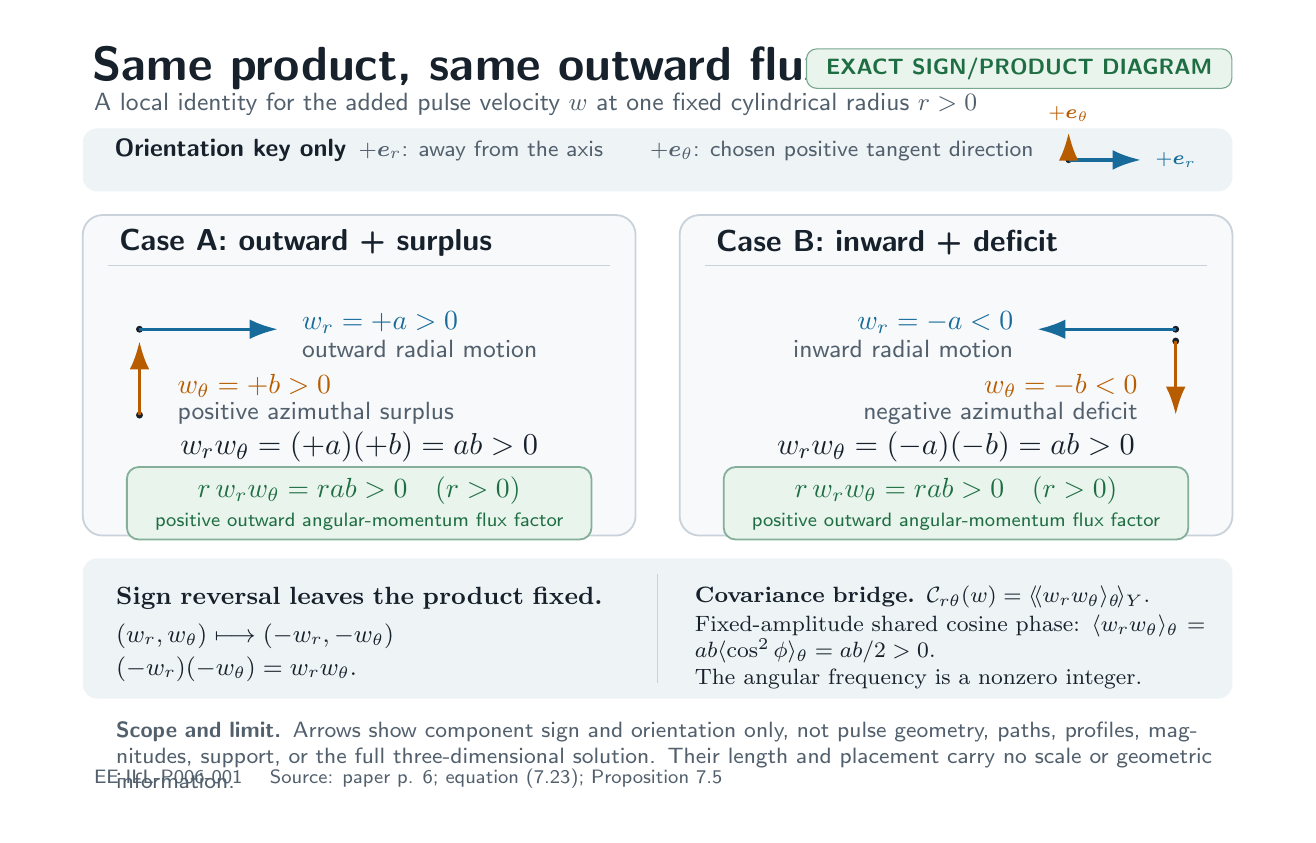
\begin{tikzpicture}[x=1cm,y=1cm]
  \path[use as bounding box] (0,0) rectangle (16,10);
  \fill[white] (0,0) rectangle (16,10);

  \node[anchor=west,font=\sffamily\bfseries\fontsize{16.5}{19.5}\selectfont,text=ink]
    at (0.7,9.48) {Same product, same outward flux};
  \node[anchor=east,draw=positive!60,fill=positivefill,rounded corners=1.3mm,
        inner xsep=2.5mm,inner ysep=1.1mm,
        font=\sffamily\bfseries\fontsize{7.7}{9.2}\selectfont,text=positive]
    at (15.3,9.48) {EXACT SIGN/PRODUCT DIAGRAM};
  \node[anchor=west,font=\sffamily\fontsize{9.2}{11.2}\selectfont,text=muted]
    at (0.72,9.03) {A local identity for the added pulse velocity $w$ at one fixed cylindrical radius $r>0$};

  % Orientation key. This is a basis key, not a spatial flow view.
  \fill[note,rounded corners=1.8mm] (0.7,7.92) rectangle (15.3,8.72);
  \node[anchor=west,font=\sffamily\bfseries\fontsize{9.1}{11}\selectfont,text=ink]
    at (0.98,8.44) {Orientation key only};
  \node[anchor=west,font=\sffamily\fontsize{8.5}{10.4}\selectfont,text=muted]
    at (4.08,8.44) {$+\boldsymbol e_r$: away from the axis};
  \node[anchor=west,font=\sffamily\fontsize{8.5}{10.4}\selectfont,text=muted]
    at (7.78,8.44) {$+\boldsymbol e_\theta$: chosen positive tangent direction};
  \fill[ink] (13.22,8.32) circle (1.15pt);
  \draw[component arrow,radial] (13.22,8.32) -- (14.14,8.32);
  \draw[component arrow,azimuthal] (13.22,8.32) -- (13.22,8.67);
  \node[anchor=west,font=\sffamily\bfseries\fontsize{7.5}{9}\selectfont,text=radial]
    at (14.20,8.32) {$+\boldsymbol e_r$};
  \node[anchor=south,font=\sffamily\bfseries\fontsize{7.5}{9}\selectfont,text=azimuthal]
    at (13.22,8.68) {$+\boldsymbol e_\theta$};

  % Two sign cases.
  \draw[case panel] (0.7,3.55) rectangle (7.72,7.62);
  \draw[case panel] (8.28,3.55) rectangle (15.3,7.62);

  \node[anchor=west,font=\sffamily\bfseries\fontsize{11.2}{13.4}\selectfont,text=ink]
    at (1.04,7.27) {Case A: outward + surplus};
  \node[anchor=west,font=\sffamily\bfseries\fontsize{11.2}{13.4}\selectfont,text=ink]
    at (8.62,7.27) {Case B: inward + deficit};
  \draw[line,line width=.55pt] (1.02,6.98) -- (7.40,6.98);
  \draw[line,line width=.55pt] (8.60,6.98) -- (14.98,6.98);

  % Case A radial component.
  \fill[ink] (1.42,6.17) circle (1.25pt);
  \draw[component arrow,radial] (1.42,6.17) -- (3.18,6.17);
  \node[anchor=west,font=\sffamily\bfseries\fontsize{10}{12}\selectfont,text=radial]
    at (3.36,6.26) {$w_r=+a>0$};
  \node[anchor=west,label text,text width=3.6cm,align=left]
    at (3.36,5.92) {outward radial motion};

  % Case A azimuthal component.
  \fill[ink] (1.42,5.08) circle (1.25pt);
  \draw[component arrow,azimuthal] (1.42,5.08) -- (1.42,6.02);
  \node[anchor=west,font=\sffamily\bfseries\fontsize{10}{12}\selectfont,text=azimuthal]
    at (1.78,5.45) {$w_\theta=+b>0$};
  \node[anchor=west,label text,text width=4.7cm,align=left]
    at (1.78,5.10) {positive azimuthal surplus};

  \node[math text] at (4.21,4.68)
    {$w_rw_\theta=(+a)(+b)=ab>0$};
  \node[result box,minimum width=5.9cm,minimum height=.76cm,align=center,
        font=\fontsize{10.1}{11.8}\selectfont,text=positive]
    at (4.21,3.96) {$r\,w_rw_\theta=rab>0\quad(r>0)$\\[-.4mm]
      {\sffamily\fontsize{7.1}{8.5}\selectfont positive outward angular-momentum flux factor}};

  % Case B radial component.
  \fill[ink] (14.58,6.17) circle (1.25pt);
  \draw[component arrow,radial] (14.58,6.17) -- (12.82,6.17);
  \node[anchor=east,font=\sffamily\bfseries\fontsize{10}{12}\selectfont,text=radial]
    at (12.64,6.26) {$w_r=-a<0$};
  \node[anchor=east,label text,text width=3.6cm,align=right]
    at (12.64,5.92) {inward radial motion};

  % Case B azimuthal component.
  \fill[ink] (14.58,6.02) circle (1.25pt);
  \draw[component arrow,azimuthal] (14.58,6.02) -- (14.58,5.08);
  \node[anchor=east,font=\sffamily\bfseries\fontsize{10}{12}\selectfont,text=azimuthal]
    at (14.22,5.45) {$w_\theta=-b<0$};
  \node[anchor=east,label text,text width=4.7cm,align=right]
    at (14.22,5.10) {negative azimuthal deficit};

  \node[math text] at (11.79,4.68)
    {$w_rw_\theta=(-a)(-b)=ab>0$};
  \node[result box,minimum width=5.9cm,minimum height=.76cm,align=center,
        font=\fontsize{10.1}{11.8}\selectfont,text=positive]
    at (11.79,3.96) {$r\,w_rw_\theta=rab>0\quad(r>0)$\\[-.4mm]
      {\sffamily\fontsize{7.1}{8.5}\selectfont positive outward angular-momentum flux factor}};

  % Algebraic bridge to the covariance used later in the proof.
  \fill[note,rounded corners=1.8mm] (0.7,1.48) rectangle (15.3,3.26);
  \node[anchor=north west,text width=6.65cm,
        font=\fontsize{8.9}{10.5}\selectfont,text=ink,align=left]
    at (1.00,3.02) {\textbf{Sign reversal leaves the product fixed.}\\[1.1mm]
      $\displaystyle (w_r,w_\theta)\longmapsto(-w_r,-w_\theta)$\\[.5mm]
      $\displaystyle (-w_r)(-w_\theta)=w_rw_\theta.$};
  \draw[line,line width=.55pt] (8.00,1.68) -- (8.00,3.06);
  \node[anchor=north west,text width=6.65cm,
        font=\fontsize{8.0}{9.3}\selectfont,text=ink,align=left]
    at (8.35,3.03) {\textbf{Covariance bridge.}
      $\mathcal C_{r\theta}(w)=\langle\!\langle w_rw_\theta\rangle_\theta\!\rangle_Y$.\\[.35mm]
      Fixed-amplitude shared cosine phase:
      $\langle w_rw_\theta\rangle_\theta=ab\langle\cos^2\phi\rangle_\theta=ab/2>0$.\\[.25mm]
      The angular frequency is a nonzero integer.};

  \node[anchor=north west,text width=14.0cm,
        font=\sffamily\fontsize{7.6}{9.2}\selectfont,text=muted,align=left]
    at (1.00,1.30) {\textbf{Scope and limit.} Arrows show component sign and orientation only, not pulse geometry, paths, profiles, magnitudes, support, or the full three-dimensional solution. Their length and placement carry no scale or geometric information.};
  \node[anchor=south west,font=\sffamily\fontsize{7.2}{8.8}\selectfont,text=muted]
    at (0.72,0.22) {EE-ILL-P006-001 \quad Source: paper p. 6; equation (7.23); Proposition 7.5};
\end{tikzpicture}
\end{document}
